% Results
The network architecture and results of the training process are presented in this section. First, the results of the training process, and then the work to expand the network to work well with experimental data.

\section{Training with Simulation Data}
The 1000 simulated XANES spectra were first loaded into a pandas dataframe \cite{pandas-1} \cite{pandas-2} of shape $ 1000\times82 $. Each of the 82 columns represents a discrete energy value, and each row represents the absorption for a given spectrum at those energies. The dataset was split into training and testing groups according to an 80-20 random split, respectively. All columns were then scaled via the standard scalar.

\begin{figure}
    \centering
    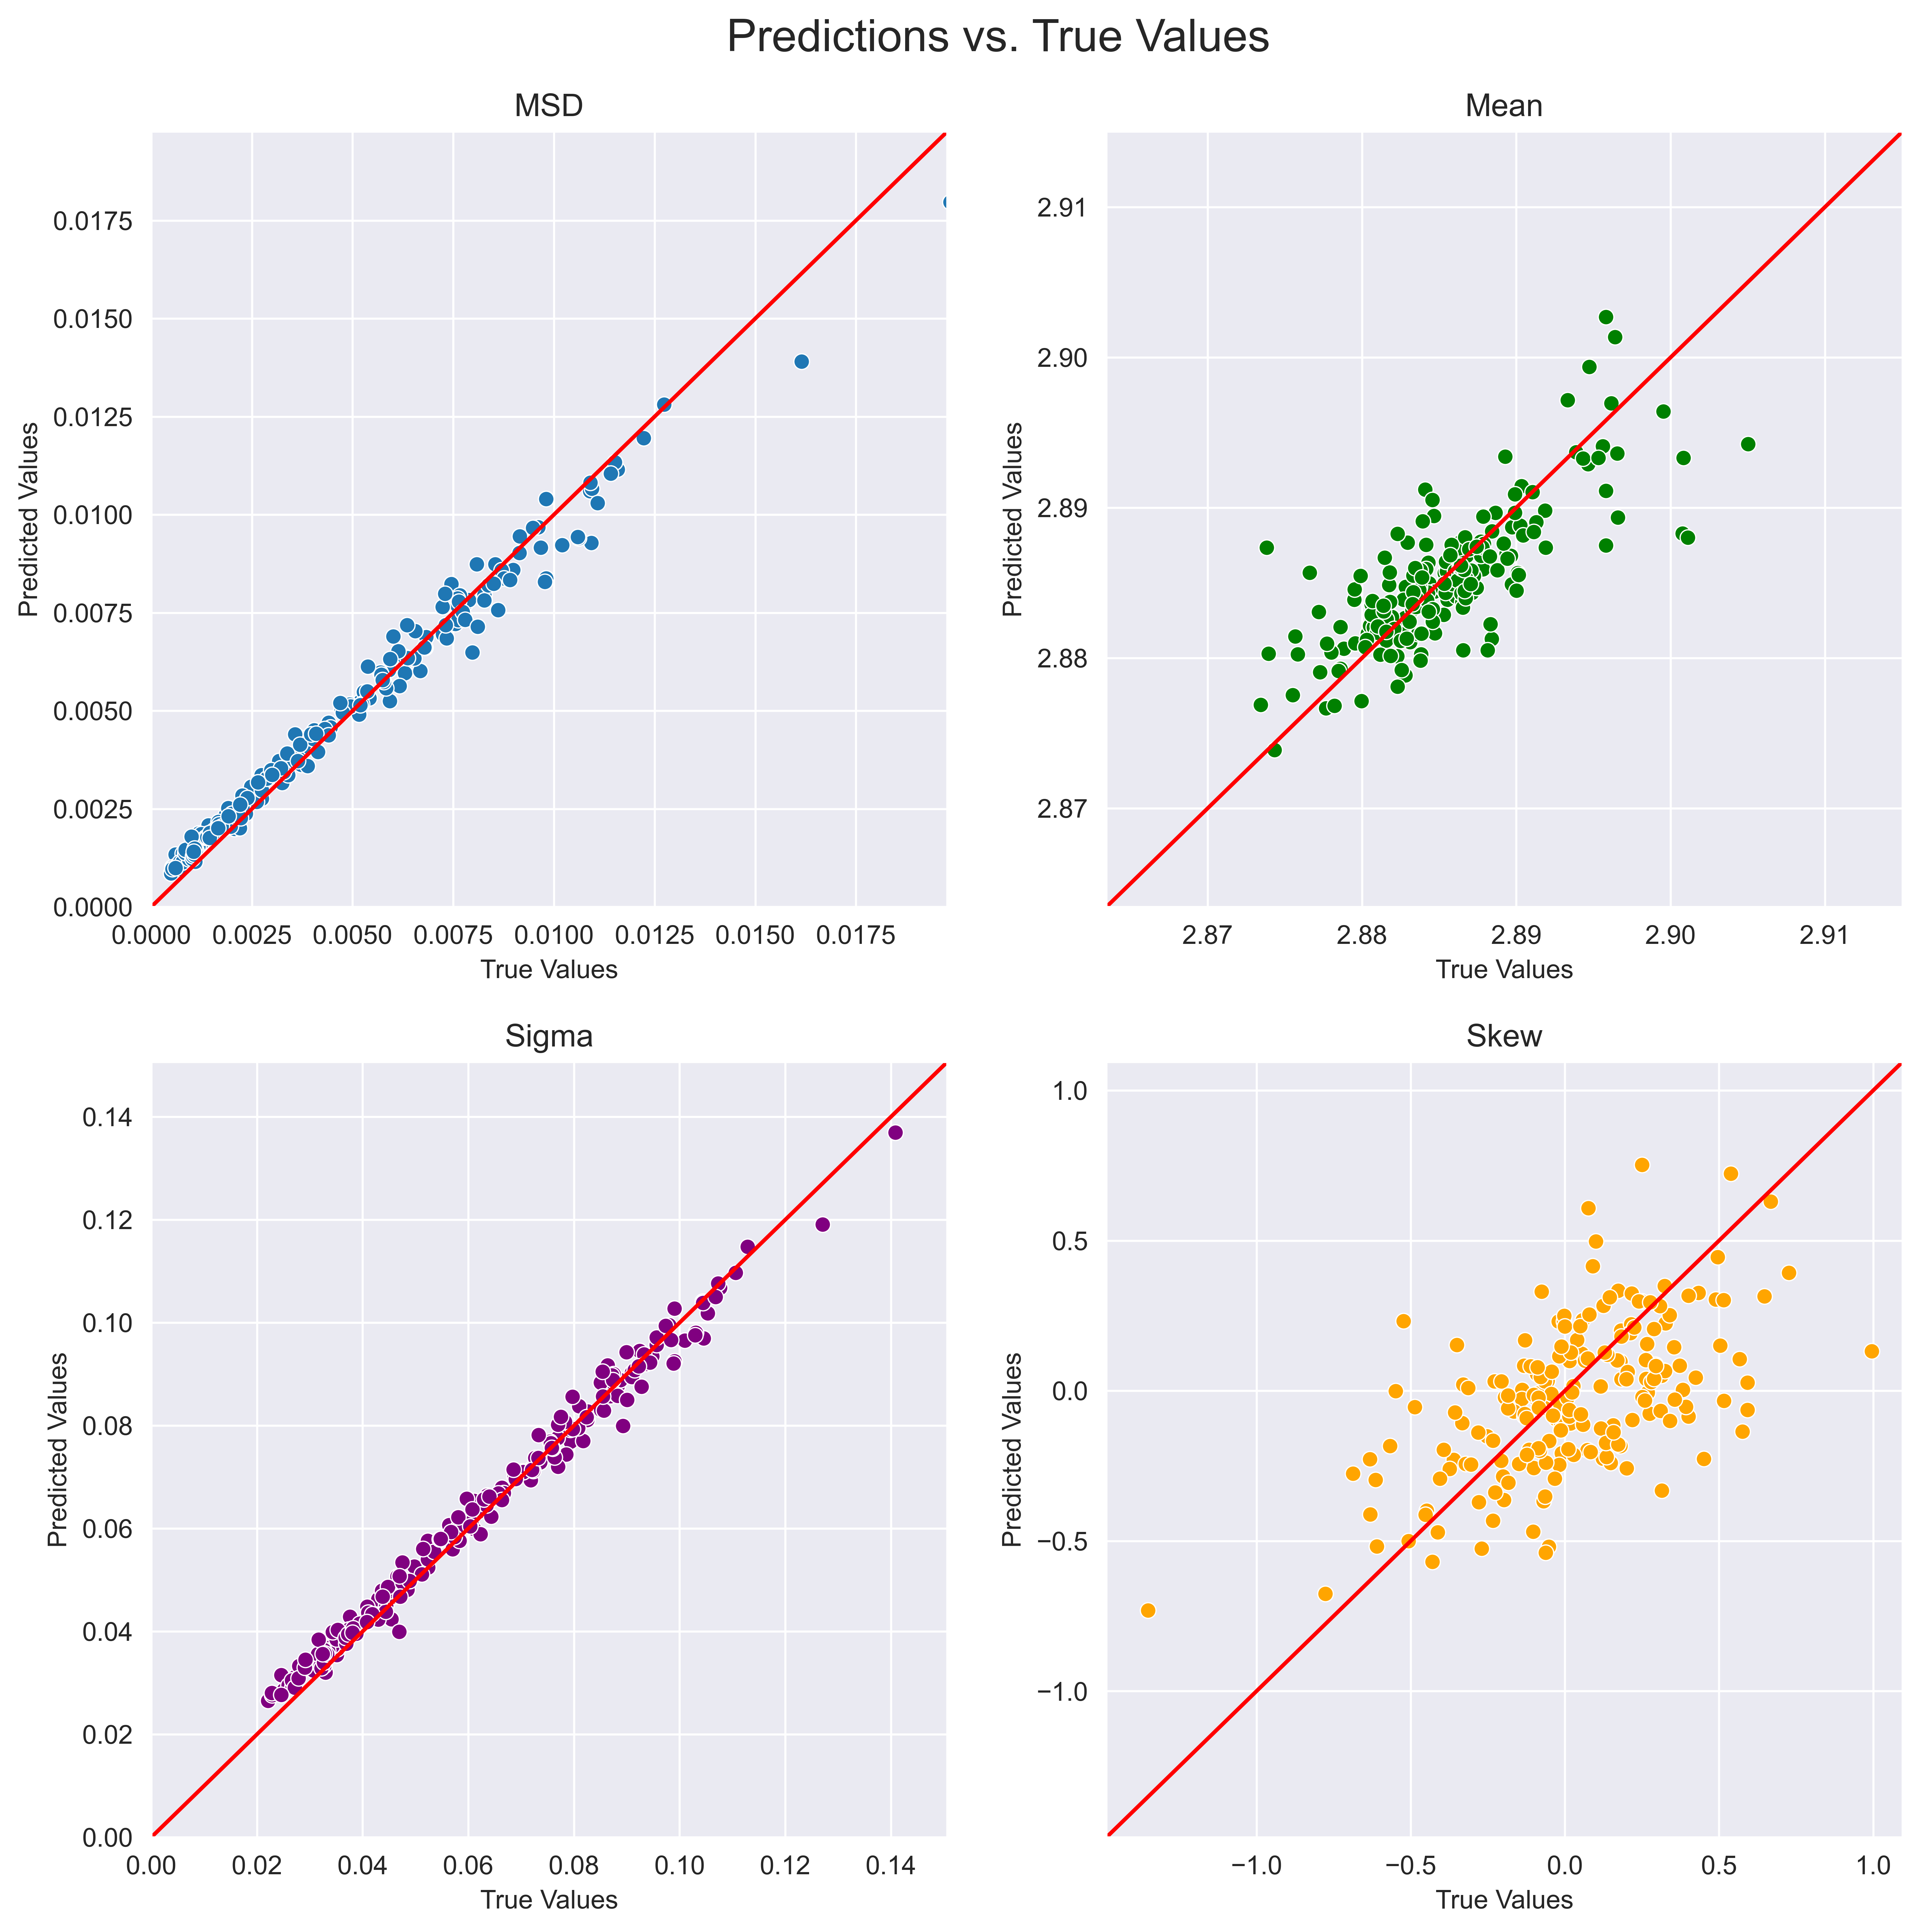
\includegraphics[width=\linewidth]{Chapters/Figures/pa_train-test (3).png}
    \caption{One version of the neural network has four output nodes: MSD, Sigma, Mean, and Kurtosis. Sigma is just the square root of the MSD and was included during training to affirm the patterns recognized by the network.}
    \label{fig:train-test-split-all4}
\end{figure}

\section{Experimental Data} \label{ch:results}
Training the neural network entirely on simulation data and then making predictions on experimental data is unlikely to provide quality results. T


\begin{figure}
    \centering
    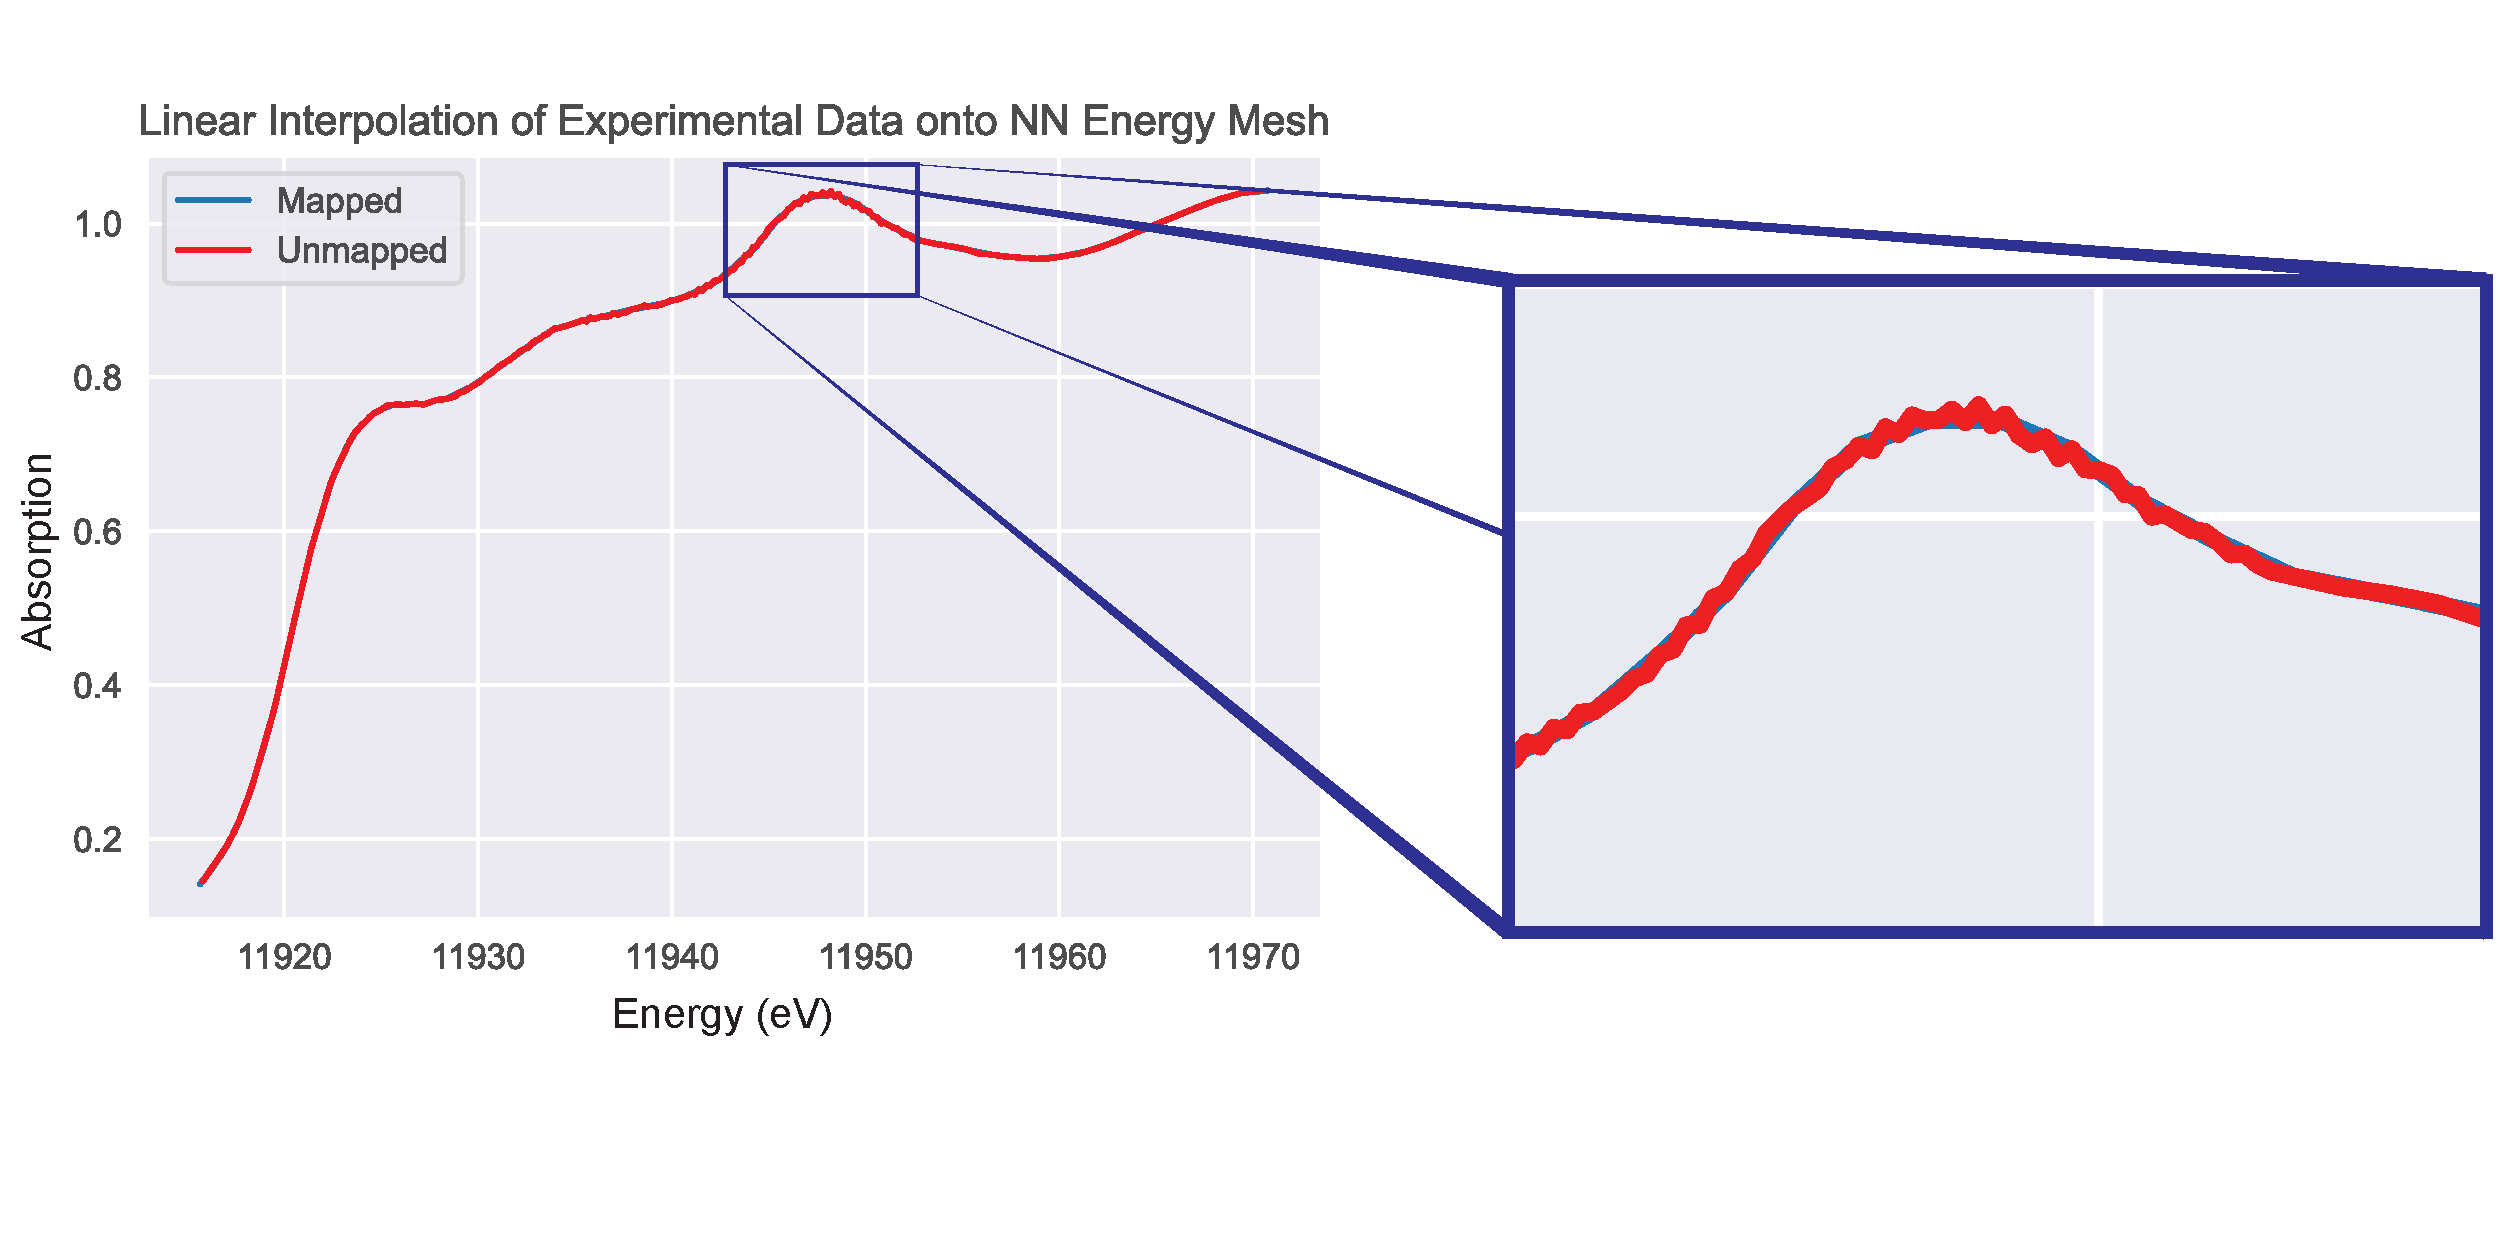
\includegraphics[width=\linewidth]{Chapters/Figures/quality-of-interpolation-figure.pdf}
    \caption[Experimental Data Interpolation]{The experimental data is measured as a function of different energy values than the ones on which the neural network is trained. Consequently, the experimental spectrum must be mapped onto the proper energy mesh via linear interpolation.}
    \label{fig:interpolation}
\end{figure}

\subsection{Data Augmentation}

\begin{figure}
    \centering
    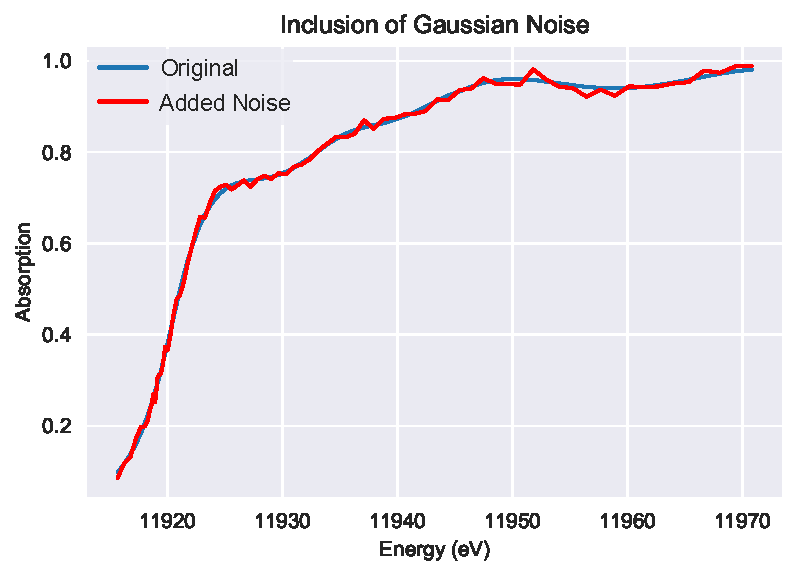
\includegraphics[width=\linewidth]{Chapters/Figures/gaussian-noise-data-aug.pdf}
    \caption[Data Augmentation: Gaussian Noise]{Gaussian Noise is added to the spectra to increase the variance of the training data. This helps the network to learn the low-level features of the spectra and ignore artifacts not caused by structural disorder. For demonstration purposes, the scale of the noise in this figure has been increased beyond what was used in training.}
    \label{fig:data-aug-gauss-noise}
\end{figure}

\begin{figure}
    \centering
    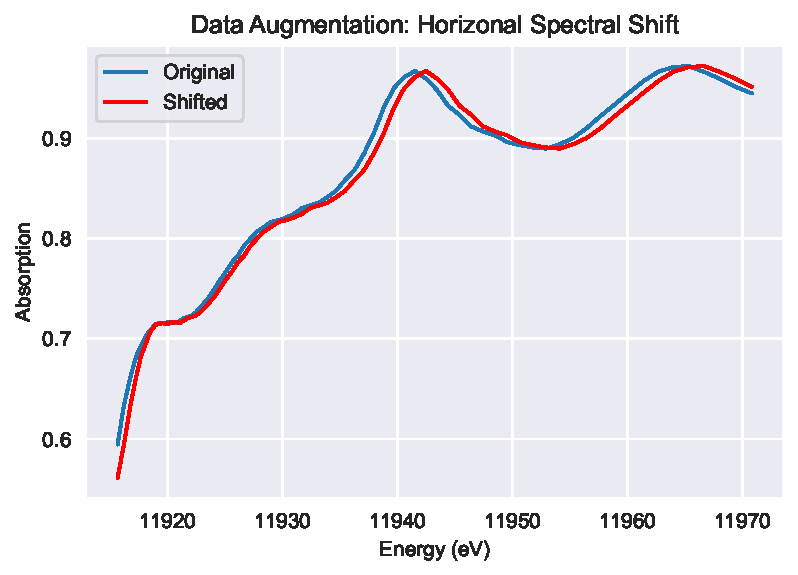
\includegraphics[width=\linewidth]{Chapters/Figures/data-aug-shift-pt75wieght.pdf}
    \caption[Data Augmentation: Horizontal Shift]{...}
    \label{fig:data-aug-hor}
\end{figure}
